% Intestazione
\fancyhead[L]{4 \hspace{0.2cm} Cruscotto di valutazione della qualità} % Testo a sinistra


\section{Cruscotto di valutazione della qualità}
\label{sec:Cruscotto di valutazione della qualità}

\vspace{0.5cm}

\subsection{Varianza dell'impegno orario}
\label{subsec:Varianza dell'impegno orario}

\begin{figure}[h] 
    \centering
    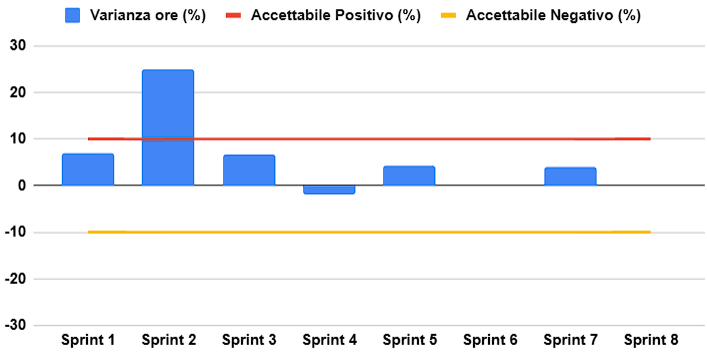
\includegraphics[width=\textwidth]{Varianza dell'impegno orario.png}
    \caption{Varianza dell'impegno orario per sprint}
    \label{fig: Varianza dell'impegno orario}
\end{figure}

\section*{Analisi}

Analizzando i valori riportati nel grafico, è riscontrabile un miglioramento nel produrre
preventivi orari vicini ai rispettivi consuntivi nel corso dell'andamento del progetto. Questo è dovuto alla scarsa esperienza iniziale del team
nel preventivare il tempo necessario per lo svolgimento delle attività nella \emph{RTB}\textsubscript{\textbf{\textit{G}}}, capacità che poi è migliorata di molto nel corso della \emph{PB}\textsubscript{\textbf{\textit{G}}}. Il picco negativo si è manifestato nella seconda sprint, dove il team ha incontrato difficoltà
nel modellare i \emph{Diagrammi dei Casi d'uso}\textsubscript{\textbf{\textit{G}}} e nel redigere i corrispettivi requisiti.
Con il progredire delle sprint, il team ha acquisito maggiore esperienza nel preventivare
il tempo necessario per lo svolgimento delle attività, riuscendo ad ottenere un valore di varianza oraria nullo, corrispondente al valore ottimo, nella sesta e nell'ottava e ultima sprint della \emph{PB}.

\newpage

\subsection{Varianza di budget}
\label{subsec:Varianza di budget}

\begin{figure}[h] 
    \centering
    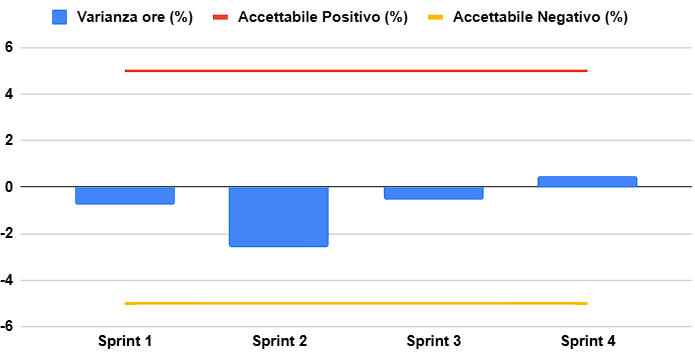
\includegraphics[width=\textwidth]{Varianza di budget.png}
    \caption{Varianza di budget per sprint} 
    \label{fig: Varianza di budget}
\end{figure}

\section*{Analisi}

Dall’analisi del grafico è immediato osservare che i valori di varianza di budget sono mediamente
peggiorati nel passaggio da \emph{RTB} a \emph{PB}, nonostante la varianza oraria sia rimasta quasi costante. In particolare, nella Sprint 5 il team ha avuto difficoltà nell'attività di progettazione, ed allora ha concentrato la maggioranza delle forze su quest'ultima, che rappresenta una delle attività più costose del progetto: ciò ha comportato un aumento dei costi rispetto al preventivo, pur senza un incremento delle ore. Il team ha poi recuperato nella Sprint 6 e nella Sprint 7, dove il difetto è stato l'opposto: il team ha ottenuto un risparmio di budget rispetto al preventivo, poichè gli sforzi per la progettazione nella Sprint 5 hanno dato i loro frutti, consentendo di risparmiare denaro nelle sprint successive. Infine, nella Sprint 8, l'ultima sprint, il team è riuscito a mantenere esattamente il budget preventivato, ottenendo un valore di varianza di budget pari a 0, e ciò dimostra l'acquisizione di esperienza avvenuta nel corso della \emph{PB}.

\newpage

\subsection{Estimate to Complete ed Estimate at Completion}
\label{subsec:Estimate to Complete ed Estimate at Completion}

\begin{figure}[h] 
    \centering
    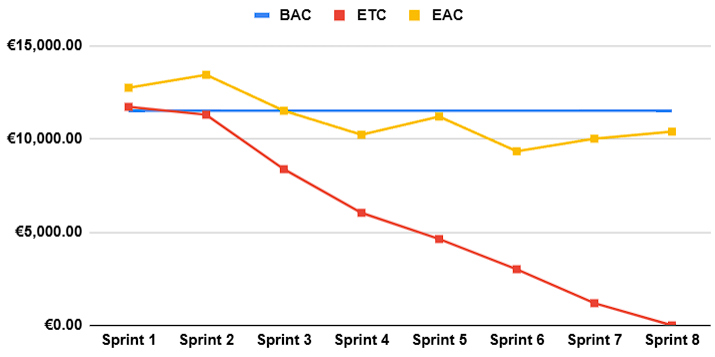
\includegraphics[width=\textwidth]{Estimate to Complete ed Estimate at Completion.png}
    \caption{Progressione Estimate to Complete e Estimate at Completion in relazione al Budget at Completion} 
    \label{fig: Estimate to Complete ed Estimate at Completion}
\end{figure}

\section*{Analisi}

Dall’analisi del grafico è immediato osservare come i valori siano andati a migliorare
nel corso delle sprint. In particolare, l’Estimate at Completion dopo la quarta sprint
è sempre stato addirittura migliore del preventivo dei costi stilato nella candidatura iniziale. Per il suddetto
contrattempo dei casi d'uso, anche in questo grafico si evidenzia l'aumento dei costi tra la prima
e la seconda sprint, per poi stabilizzarsi e migliorare nel corso delle sprint successive. La produttività nel corso delle ultime 5 sprint ha consentito al team di risparmiare risorse, ottenendo sempre un valore di Estimate at Completion inferiore al Budget at Completion. Per quanto riguarda l'Estimate to Complete, dopo una leggera difficoltà iniziale, esso procede scendendo regolarmente fino a zero, a dimostrazione dell'efficienza del team nel risparmiare risorse e nel completare il progetto con successo.

\newpage

\subsection{Planned Value, Earned Value e Actual Cost}
\label{subsec:Planned Value, Earned Value e Actual Cost}

\begin{figure}[h] 
    \centering
    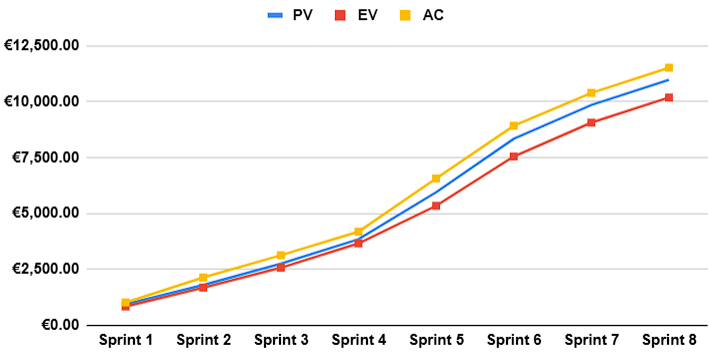
\includegraphics[width=\textwidth]{Planned Value, Earned Value e Actual Cost.png}
    \caption{Progressione Planned Value, Earned Value e Actual Cost} 
    \label{fig: Planned Value, Earned Value e Actual Cost}
\end{figure}

\section*{Analisi}

Analizzando il grafico, si può notare come i tre valori abbiano sempre progredito seguendo una
proporzione costante. In particolare, l’Actual Cost è stato sempre superiore al Planned Value,
il quale a sua volta è stato sempre superiore all’Earned Value. Questo è dovuto al fatto che
il team ha impiegato leggermente più tempo del previsto per svolgere leggermente meno attività preventivate.  
In particolare, nelle ultime sprint vi è stato un leggero distacco tra l'Earned Value e gli altri due valori, dovuto al fatto che il team, pur rispettando il numero di ore, ha incontrato qualche difficoltà nelle attività di progettazione e programmazione.

\newpage

\subsection{Schedule Variance e Cost Variance}
\label{subsec:Schedule Variance e Cost Variance}

\begin{figure}[h] 
    \centering
    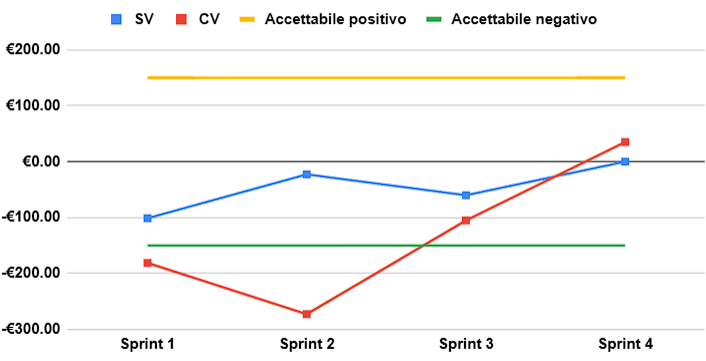
\includegraphics[width=\textwidth]{Schedule Variance e Cost Variance.png}
    \caption{Progressione Schedule Variance e Cost Variance} 
    \label{fig: Schedule Variance e Cost Variance}
\end{figure}

\section*{Analisi}

Dal grafico, risulta ancora evidente come il team abbia avuto difficoltà nel
rispettare i costi preventivati, seppur abbia mediamente rispettato il numero di ore. La Schedule Variance e la Cost Variance sono infatti
risultate sempre negative, tranne nelle ultime sprint delle revisioni \emph{RTB} e \emph{PB}, nelle quali si nota un miglioramento
significativo. I risultati peggiori si registrano nella seconda sprint e nella quinta sprint per i suddetti
motivi, legati rispettivamenti all'analisi dei requisiti e alla progettazione: infatti, queste ultime rappresentano due tra le attività più costose del progetto, e quindi quando il team si è concentrato su di esse i costi sono saliti. Questo è il motivo per cui, seppur il numero di ore non sia mai stato largamente superato, la distribuzione delle stesse verso attività costose ha comportato una marcata varianza dei costi. Tuttavia, fortunatamente la varianza è stata bilanciata verso il termine delle revisioni, poichè le ore in quei periodi sono state dedicate ad attività come la codifica e la verifica, che sono meno costose.

\newpage

\subsection{Schedule Performance Index e Cost Performance Index}
\label{subsec:Schedule Performance Index e Cost Performance Index}

\begin{figure}[h] 
    \centering
    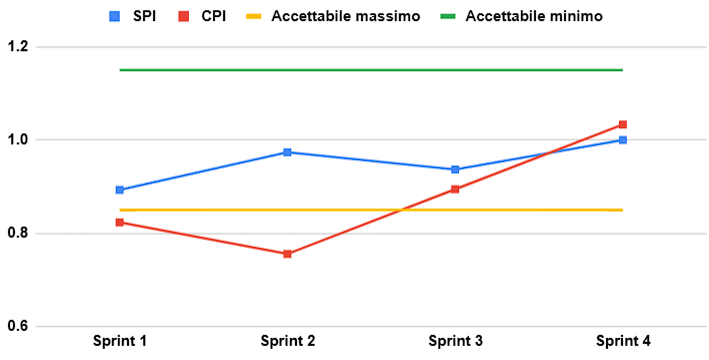
\includegraphics[width=\textwidth]{Schedule Performance Index e Cost Performance Index.png}
    \caption{Progressione Schedule Performance Index e Cost Performance Index} 
    \label{fig: Schedule Performance Index e Cost Performance Index}
\end{figure}

\section*{Analisi}

Similmente a quanto riscontrabile dall’analisi del grafico di Schedule e Cost Variance, anche
il valore del Cost Performance Index è sceso sotto la soglia accettabile nella 
sprint 2 e nella sprint 5, per poi recuperare nelle sprint terminali delle revisioni \emph{RTB} e \emph{PB}: ciò è dovuto, come suddetto, alle attività di analisi dei requisiti e di progettazione. Nella quarta sprint e nella settima sprint, invece, il team
ha addirittura raggiunto un valore di Cost Performance Index superiore a 1, indicando
che sono state spese meno risorse rispetto a quanto preventivato per lo svolgimento delle
attività meno costose previste per le sprint finali.\\
Il valore dello Schedule Performance Index è invece sempre stato inferiore a 1, addirittura scendendo sotto la soglia accettabile nella sprint 5, a indicare la difficoltà che il team ha avuto nel preventivare le ore in tale sprint, in cui, oltre alle difficoltà di progettazione, è da segnalare che metà gruppo è stato impegnato nello studio per il secondo appello di Ingegneria del Software.
Nelle sprint 4, 7 ed 8, invece, lo Schedule Performance Index è risultato pari a 1, indicando che, come suddetto, verso la fine delle revisioni, il team è riuscito a svolgere
con successo tutte le attività preventivate.

\newpage

\subsection{Misure di mitigazione insufficienti}
\label{subsec:Misure di mitigazione insufficienti}

\begin{figure}[h] 
    \centering
    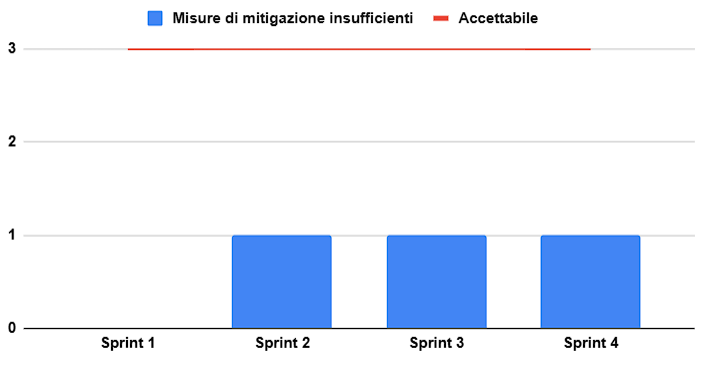
\includegraphics[width=\textwidth]{Misure di mitigazione insufficienti.png}
    \caption{Progressione occorrenza di rischi con misure mitigative insufficienti} 
    \label{fig: Misure di mitigazione insufficienti}
\end{figure}

\section*{Analisi}

Durante il progetto, il team ha riscontrato difficoltà nell'applicare alcune misure di mitigazione
per i rischi individuati.
\begin{itemize}
    \item In particolare, per gestire i rischi legati alla comunicazione interna nella seconda sprint, è stato necessario che 
    tutti i membri del team si accordassero sia sulla sintassi che sulla semantica nella modellazione dei casi d'uso;
    \item Successivamente, per affrontare i rischi di non conformità rispetto agli impegni dichiarati nella terza sprint, si è 
    dovuto considerare l'impatto delle vacanze natalizie e dello studio per la sessione d'esami;
    \item Nella quarta sprint, per gestire i rischi legati alla complessità delle tecnologie, è emersa la necessità di 
    un aiuto reciproco nella programmazione. La spartizione iniziale dei compiti prevedeva esploratori solitari per ciascuna 
    tecnologia e una bassa condivisione delle conoscenze. Questo ha reso difficile lavorare in gruppo e chiedere aiuto ai compagni 
    al momento dell'\emph{implementazione}\textsubscript{\textbf{\textit{G}}} del \emph{PoC}\textsubscript{\textbf{\textit{G}}};
    \item Infine, nella quinta sprint, il team ha dovuto affrontare il rischio legato agli impegni accademici, poichè metà del gruppo ha dovuto studiare per il secondo appello di Ingegneria del Software. Questo ha comportato un rallentamento delle attività, che è stato mitigato con una ridistribuzione dei compiti e con un maggiore supporto reciproco.
\end{itemize}
Fortunamente, si può notare come il team abbia saputo reagire in modo efficace a queste difficoltà, riuscendo a presentare misure sufficienti per ciascuna di esse nelle ultime 3 sprint.

\newpage

\subsection{Rischi inattesi}
\label{subsec:Rischi inattesi}

\begin{figure}[h] 
    \centering
    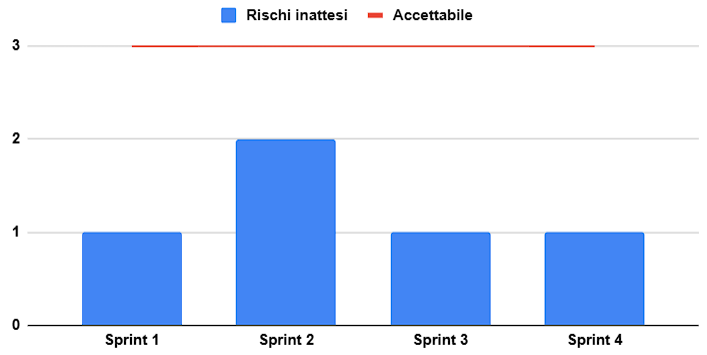
\includegraphics[width=\textwidth]{Rischi inattesi.png}
    \caption{Progressione occorrenza di rischi inattesi} 
    \label{fig: Rischi inattesi}
\end{figure}

\section*{Analisi}

Come osservabile dai valori riportati dal grafico, l’ampia analisi dei rischi effettuata a inizio progetto è stata soddisfacente. 
L'unica problematica primaria riconoscibile come rischio non già presente nella sezione dedicata del \emph{Piano di progetto}\textsubscript{\textbf{\textit{G}}} è stata riscontrata solo al termine dei lavori: 
si tratta dell'assenza di un professore, in particolare del professor Cardin, nell'ultima settima di marzo, che ci ha fatto posticipare il termine del progetto. 
Fortunatamente, essendo questa problematica emersa solamente nel periodo finale del progetto, non ha causato ritardi su attività precedenti alla revisione \emph{Product Baseline}\textsubscript{\textbf{\textit{G}}}, 
però potrebbe causare ritardi in caso emergano errori a valle della revisione.
Inoltre, questa situazione ha costretto un componente del gruppo a posticipare l'inizio del proprio tirocinio, dimostrando l'impatto che i rischi inattesi possono avere sulla pianificazione personale dei membri del team.\\
Il team si è trovato inizialmente impreparato, ma ha poi saputo reagire in modo efficace, 
riuscendo a completare la documentazione con maggiore calma e a terminare le attività di progetto 
senza incidere significativamente sul costo orario.



\newpage

\subsection{Requisiti soddisfatti}
\label{subsec:Requisiti soddisfatti}

\begin{figure}[h] 
    \centering
    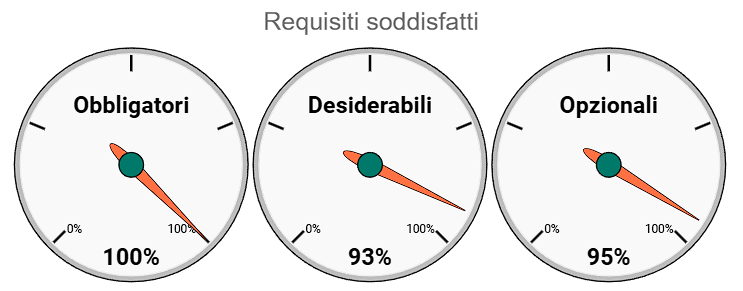
\includegraphics[width=\textwidth]{Requisiti soddisfatti.png}
    \caption{Requisiti obbligatori, desiderabili e opzionali soddisfatti} 
    \label{fig: Requisiti soddisfatti}
\end{figure}

\section*{Analisi}
L'\emph{MVP}\textsubscript{\textbf{\textit{G}}} sviluppato nella \emph{Product Baseline} ha soddisfatto tutti i requisiti obbligatori stabiliti assieme al \emph{proponente}\textsubscript{\textbf{\textit{G}}}. Invece, non sono stati soddisfatti un requisito desiderabile e un requisito opzionale, entrambi in accordo con il proponente: il primo, relativo alla visualizzazione di un segnale di inizio dello storico dei messaggi, è stato ritenuto non necessario e troppo facilmente confondibile con un messaggio di errore, mentre il secondo, relativo alla funzionalità di selezione di alcune domande proposte per iniziare la conversazione, si è ritrovato in contrasto con la funzionalità dello storico, che ha reso concettualmente complesso capire quale fosse l'"inizio della conversazione", ed allora è stato scartato.

\newpage

\subsection{Indice di Gulpease}
\label{subsec:Indice di Gulpease}


\begin{figure}[h!] 
    \centering
    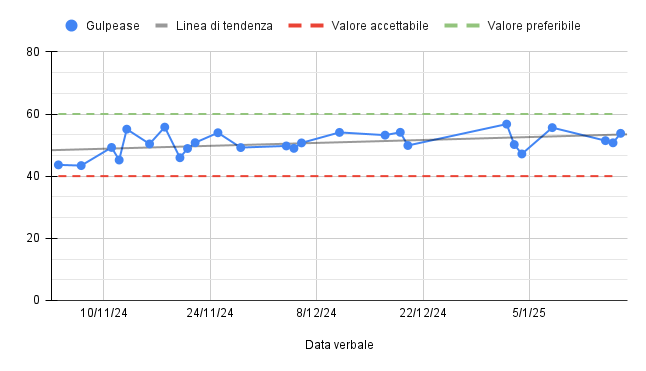
\includegraphics[width=\textwidth]{Gulpease verbali RTB.png}
    \caption{Andamento indice di Gulpease nei verbali - RTB} 
    \label{fig: Andamento Gulpease verbali RTB}
\end{figure}

\begin{figure}[h!] 
    \centering
    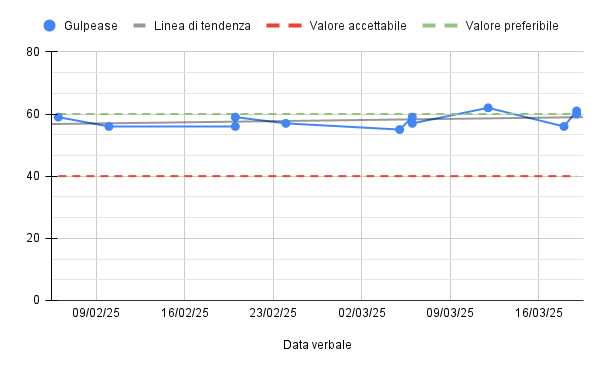
\includegraphics[width=\textwidth]{Gulpease verbali PB.png}
    \caption{Andamento indice di Gulpease nei verbali - PB} 
    \label{fig: Andamento Gulpease verbali PB}
\end{figure}

\begin{figure}[h!]
    \centering

    \begin{minipage}{.4\textwidth}
        \centering
        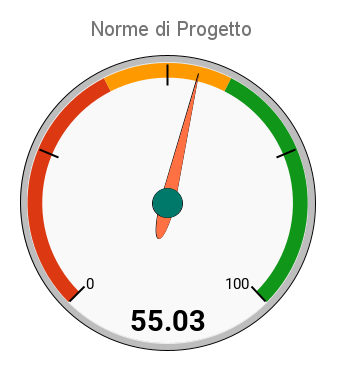
\includegraphics[width=.8\linewidth]{Gulpease Norme di Progetto.png}
        \caption{Indice di Gulpease Norme di Progetto}
        \label{fig:Gulpease Norme Progetto}
    \end{minipage}
    \hfill
    \begin{minipage}{.4\textwidth}
        \centering
        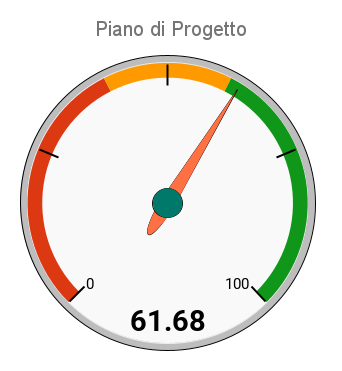
\includegraphics[width=.8\linewidth]{Gulpease Piano di Progetto.png}
        \caption{Indice di Gulpease Piano di Progetto}
        \label{fig:Gulpease Piano Progetto}
    \end{minipage}

\end{figure}

\begin{figure}[H]
    \centering

    \begin{minipage}{.4\textwidth}
        \centering
        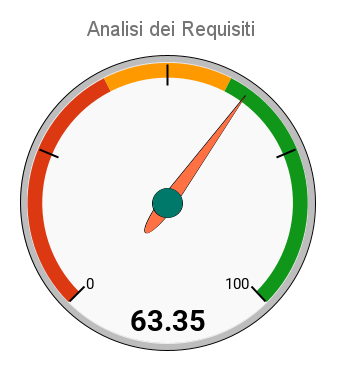
\includegraphics[width=.8\linewidth]{Gulpease Analisi dei Requisiti.png}
        \caption{Indice di Gulpease Analisi dei Requisiti}
        \label{fig:Gulpease Analisi Requisiti}
    \end{minipage}%
    \hfill
    \begin{minipage}{.4\textwidth}
        \centering
        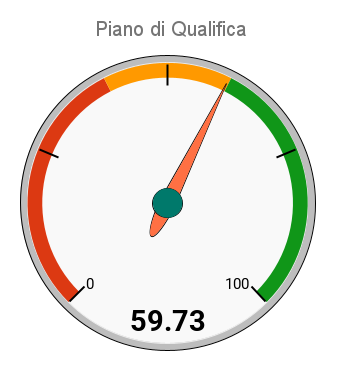
\includegraphics[width=.8\linewidth]{Gulpease Piano di Qualifica.png}
        \caption{Indice di Gulpease Piano di Qualifica}
        \label{fig:Gulpease Piano Qualifica}
    \end{minipage}

\end{figure}

\begin{figure}[H]
    \centering

    \begin{minipage}{.4\textwidth}
        \centering
        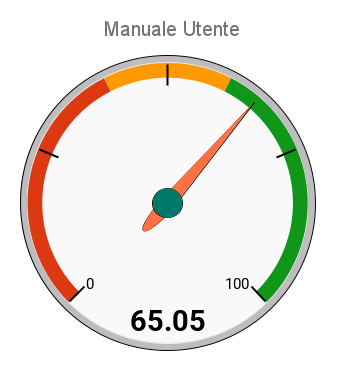
\includegraphics[width=.8\linewidth]{Gulpease Manuale Utente.png}
        \caption{Indice di Gulpease Manuale Utente}
        \label{fig:Gulpease Manuale Utente}
    \end{minipage}%
    \hfill
    \begin{minipage}{.4\textwidth}
        \centering
        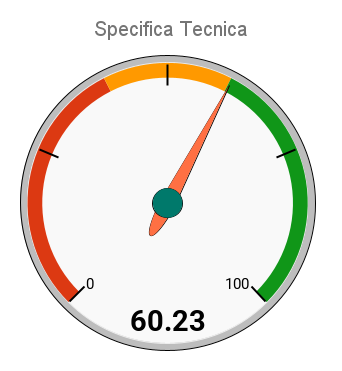
\includegraphics[width=.8\linewidth]{Gulpease Specifica Tecnica.png}
        \caption{Indice di Gulpease Specifica Tecnica}
        \label{fig:Gulpease Specifica Tecnica}
    \end{minipage}

\end{figure}


\newpage

\section*{Analisi}

Questi valori mostrano che la documentazione è generalmente accessibile e comprensibile, 
dato che tutti i documenti superano la soglia accettabile di 40 nell'\emph{indice di Gulpease}\textsubscript{\textbf{\textit{G}}}, 
con la maggior parte dei valori che si avvicinano al "valore preferibile" di 60. 
In particolare, è utile notare come, nel grafico relativo all'andamento dell'indice di Gulpease dei verbali durante la \emph{RTB}\textsubscript{\textbf{\textit{G}}}, la linea di tendenza sia crescente,
il che mostra un generale miglioramento da parte del gruppo nella qualità della documentazione prodotta.
Questa tendenza è stata confermata nella \emph{Product Baseline}\textsubscript{\textbf{\textit{G}}},
durante la quale il valore dell'indice per i verbali ha avuto una crescita meno evidente, ma si è stabilizzato attorno al "valore preferibile" di 60.

\newpage

\subsection{Code Coverage}
\label{subsec:Code Coverage}

\begin{figure}[h] 
    \centering
    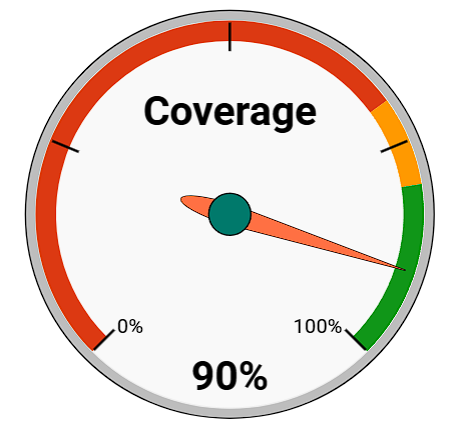
\includegraphics[width=.4\textwidth]{Code Coverage.png}
    \caption{Code Coverage} 
    \label{fig: Code Coverage}
\end{figure}

\section*{Analisi}
La \emph{Code Coverage}\textsubscript{\textbf{\textit{G}}} è un indicatore che misura la percentuale di codice sorgente coperto dai \emph{test}\textsubscript{\textbf{\textit{G}}}. Nel tentativo di migliorare questo indicatore, il team ha scritto \emph{test di unità}\textsubscript{\textbf{\textit{G}}} e \emph{test di integrazione}\textsubscript{\textbf{\textit{G}}} per ogni classe del \emph{backend}\textsubscript{\textbf{\textit{G}}} e per ogni componente del \emph{frontend}\textsubscript{\textbf{\textit{G}}}, raggiungendo un valore di coverage pari al 90\% per entrambi. Questo è un buon risultato, che dimostra l'efficacia dei test effettuati, e soprattutto che soddisfa la soglia minima richiesta dal \emph{proponente} \emph{AzzurroDigitale}\textsubscript{\textbf{\textit{G}}}, cioè 70/80\% di copertura, che il team è stato in grado anche di superare.
